\documentclass[12pt,a4paper]{article}

% Paquetes esenciales para el formato y tablas
\usepackage[utf8]{inputenc}
\usepackage[spanish]{babel}
\usepackage{geometry}
\geometry{a4paper, margin=2.5cm}
\usepackage{graphicx}
\usepackage{tabularx}
\usepackage{booktabs}
\usepackage{multirow}
\usepackage{hyperref}
\usepackage[table]{xcolor}
\usepackage{float}

\hypersetup{
    colorlinks=true,
    linkcolor=blue,
    urlcolor=cyan,
}

% Comandos personalizados para notas o ejemplos que debes borrar
\newcommand{\instruccion}[1]{\textcolor{red}{\textit{[#1]}}}
\newcommand{\ejemplo}[1]{\textcolor{gray}{\textit{Ejemplo: #1}}}

\title{\textbf{Informe de Vigilancia Tecnológica para Trabajo de Titulación}}
\author{Gabriel Zapata Salazar y Yu Ze Zhou}
\date{\today}

\begin{document}
\sloppy
\maketitle



\section*{Definición técnica del Problema}
    \subsection*{Perfil Técnico}
        \begin{itemize}
            \item Requisitos del Sistema:  
            \begin{enumerate}
                \item \textbf{Requerimientos Funcionales:}
                    \begin{itemize}
                        \item \textbf{RF1.} Ingesta de datos: El sistema debe ser capaz de cargar y leer múltiples archivos de datos estructurados po telemetría(Archivos excel que contienen datos de las ONT, OLT, NOC).
                        \item \textbf{RF2.} Limpieza y Preprocesamiento: El sistema debe ejecutar ciclos periodicos para limpiar los arhivos, específicamente, manejar valores nulos, eliminar datos duplicados, coregir formatos de datos (Por ejemplo, transformar fechas a "dd-MM-yyyy"), filtrar ruido en las mediciones y datos inconsistentes.
                        \item \textbf{RF3.} Feature Engineering: El sistema debe generar nuevas variables calculadas a partir de datos ya procesados (por ejemplo, calcular calcular potencia óptica en diferentes periodos según la medición diaria).
                        \item \textbf{RF4.} Visualización de distribución: Visualizar la distribución de datos mediante gráficos y obtener valores estadísticos para la toma de decisión en la elección de los algoritmos a utilizar.
                        \item \textbf{RF5.} Entrenamiento y Validación: El sistema sistema debe permitir entrenar algoRitmos de aprendizaje automático utilizando el conjunto de datos históricos previamente pocesados y valida su rendimiento mediante técnicas como \textbf{Cross-validation}.
                        \item \textbf{RF6.} Generación de predicciones: El sistema debe evaluar los nuevos datos ingresados y emitir una probabilidad de degradación o falla por algún equipo (ONT/OLT) en algún segmento de red específico.
                        \item \textbf{RF7.} Evaluación de métricas: El sistema deberá calcular y mostrar métricas de rendimiento del modelo (Por ejemplo, Precisión, Recall, F1-Score, Matriz de confusión, entre otros). 
                    \end{itemize}
                \item \textbf{Requerimientos de Interfaces:}
                    \begin{itemize}
                        \item Interfaz de datos (Datos): El sistema equiere de una lectura de archivos locales o en un servicio de nube que sopote los fomatos \textbf{.csv}, \textbf{.xlsx} y \textbf{.xls}.
                        \item Interfaz de Salida (Resultados): El sistema deberá expotar las predicciones generadas a un formato estandarizado (por ejemplo, un archivo \textbf{.csv} con el identificador del equipo y su probabilidad de falla) para que pueda ser intepretado por la gerencia.
                        \item Interfaz de Usuario (UI): Visualizar los resultados mediante una interfaz gráfica e interactiva mediante herramientas como Jupyter Notebooks, Google Collab o procesar y exportar los datos a Power BI.
                    \end{itemize}
                \item \textbf{Requerimientos de Ambiente:}
                    \begin{itemize}
                        \item \textbf{Requerimientos de Software:} 
                        \begin{enumerate}
                            \item Python versión 3.8 o superior.
                            \item Librerías de procesamiento y modelado de datos: Pandas, numpy, matplotlib, Gym, Sckit-learning, XGBoost, pytorch, Tensorflow, dependiendo de las necesidades y arquitectura a escoger.
                            \item Sistema operativo compatible con el entorno de desarrollo (Windows/Linux).
                        \end{enumerate}
                        \item \textbf{Requerimientos de Hardware:}
                        \begin{enumerate}
                            \item \textbf{Memoria RAM:} Se recomienda tener un mínimo de 16 GB o 32 GB de RAM para el procesamiento de datos y unificación de datasets, evitando así, un cuello de botella en la limpieza de varios excels.
                            \item \textbf{Procesamiento (CPU/GPU):} La elección dependerá de la arquitectura de entrenamiento a utilizar. Procesador Multi-núcleo para paralelizar el entrenamiento o tareas de secuencias complejas de pocos núcleos, especialmente útil en técnicas de aprendizaje reforzado de algoritmos como Actor-Crítico (A2C). El uso de la GPU será de gran ventaja en el procesamiento de múltiples hilos ejecutando aritmética báscia, siendo especialmente útil en el entrenamiento de redes neuronales profundas. 
                        \end{enumerate}
                        \item \textbf{Entorno de ejecución:} Será necesario requerir un entorno de ejecución en la nube dado un volumen de datos pesado provisto. Por lo que se recomienda contar con una licencia de Google collab (existen otras opciones) que permita seleccionar un hardware con mayor capacidad de cómputo. 
                    \end{itemize}
                
            \end{enumerate}

            \item \textbf{Arquitectura del Sistema:}
            El sisguiente diagrama resume la aquitectura de alto nivel del modelo predictivo destinado para la posible detección de degradaciones en la red FTTH.
            \begin{enumerate}
                \item \textbf{Esquema General del Sistema:} 
                    \begin{figure}[H]
                        \centering
                        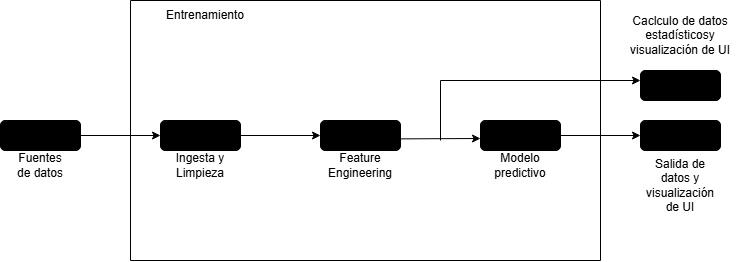
\includegraphics[width=0.8\textwidth]{Esquemas e imágenes/Arquitectura ML FTTH.png}
                    \end{figure}
                \item \textbf{Descripción de Componentes:}
                
                    \begin{table}[H]
                        \centering
                        \begin{tabularx}{\textwidth}{|p{3.5cm}|X|p{2cm}|}
                            \hline
                            \rowcolor{black} 
                            \textcolor{white}{Módulo} & \textcolor{white}{Propósito} & \textcolor{white}{Sección}  \\ \hline
                            
                            \textbf{M.1: Fuentes de datos} & El módulo extrae por telemetría estática y dinámica. Esto incluye: mediciones de potencia óptica (Rx/Tx) proveniente de las ONT, registros de estado de los puertos PON, alarmas, entre otros. & Dato 1.3 \\ \hline
                            \textbf{M.2: Ingesta y Limpieza} & El módulo realiza la consolidación de las distintas fuentes mediante identificadores en común (número serial del dispositivo/ID del cliente y el puerto lógico de la OLT). Además, se realiza una limpieza de datos cuyas acciones incluye: manejo de valores nulos, resgistros duplicados y estandarizar formatos. & Dato 2.3 \\ \hline
                            \textbf{M.3: Feature Engineering} & Crea nuevas variables matemáticas a partir de los datos históricos para ayudar al modelo a encontrar patrones de degradación. & Dato 3.3 \\ \hline
                            \textbf{M.4: Modelo predictivo} & El algoitmos de machine leaning (Por ejemplo, Random Forest, XGBoost, Redes neuronales profundas, aprendizaje refozado). Durante la fase de desarrollo, este componente aprende los patrones de falla. En producción, toma los datos nuevos y calcula la probabilidad de degradación. & Dato 3.3 \\ \hline
                            \textbf{M.5: Cálculo de datos estadísticos y visualización de UI} & A partir del entrenamiento, en esta etapa se valida el modelo evaluando métricas estadísticos, el cual será visualizado mediante una interfaz destinado a la gerencia. El interfaz mostrará las métricas previamente mencionado, además de los segmentos de red asociado a los dispositivos que pesentan una caída de servicio y su probabilidad de ocurrencia. & Dato 3.3 \\ \hline
                            \textbf{M.6: Salida de datos y visualización de UI} & Se muestra la distribución de datos tras su limpieza para entender e interpretar el compotamiento a nivel físico de la red FTTH. La visualización será mediante una interfaz desplegada para que el usuario interactúe dinámicamente. En ella se visualizan diversos gráficos acompañado de valores estadísticos. & Dato 3.3 \\ \hline
                        \end{tabularx}
                    \end{table}
                \item \textbf{Matriz de	Requisitos Funcionales y Componentes:} 
                
                    \begin{table}[H]
                        \centering
                        \begin{tabularx}{\textwidth}{|X|p{1cm}|p{1cm}|p{1cm}|p{1cm}|p{1cm}|p{1cm}|}
                            \hline
                            \rowcolor{black} 
                            \textcolor{white}{Requerimiento} & \textcolor{white}{M.1} & \textcolor{white}{M.2} & \textcolor{white}{M.3} & \textcolor{white}{M.4} & \textcolor{white}{M.5} & \textcolor{white}{M.6}  \\ \hline
                            
                            \textbf{RF1} & X & & & & & \\ \hline
                            \textbf{RF2} & & X & & & & \\ \hline
                            \textbf{RF3} & & & X & & & \\ \hline
                            \textbf{RF4} & & & & & & x \\ \hline
                            \textbf{RF5} & & & & X & & \\ \hline
                            \textbf{RF6} & & & & X & & \\ \hline
                            \textbf{RF7} & & & &  & X & \\ \hline
                        \end{tabularx}
                    \end{table}
                
            \end{enumerate}
            \item \textbf{Gestión de Riesgos:}
            \begin{enumerate}
                \item \textbf{Supuestos:}
                    \begin{itemize}
                        \item \textbf{S1-Correlación de variables:} Se asume que existe una correlación matemática real y detectable mentre los parámetros de telemetía extraídos y las degradaciones dísicas de la red antes de que se conviertan en un reclamo masivo por los clientes.
                        \item \textbf{S2-Representatividad histórica:} Se asume que los archivos Excel/CSV entregado por la jefatura contienen un historial de tiempo lo suficientemente amplio (muchos meses) para que el algoritmo pueda aprender los patrones estacionales y transitorios de las fallas.
                        \item \textbf{S3-Capacidad de procesamiento:} Se asume que los datos proporcionados podrán ser procesado con los recursos computacionales actuales sin requerir de una infraestreuctura de Big Data de alto costo.
                    \end{itemize}
                \item \textbf{Dependencias:}
                    \begin{itemize}
                        \item \textbf{D1-Entrega de datos corporativos:} El avance del cronograma depende estrictamente de que el tutor y Liberty Latinamerica proporcionen los datasets iniciales y las actualizaciones de datos en los plazos acordados.
                        \item \textbf{D2-Diccionario de datos:} Se depende de la empresa para la entrega de un glosario o diccionario de datos que explique el significado de cada columna en los Excel para realizar un feature Engineering y reducción de dimensionalidad correcto.
                        \item \textbf{D3-Validación experta:} Se depende del conocimiento del tutor para validar si las variables que el modelo considere ``importantes'' tienen sentido físico dentro de la topología FTTH real.
                    \end{itemize}
                \item \textbf{Restricciones:} 
                    \begin{itemize}
                        \item \textbf{R1-Restricción de tiempo:} El proyecto está acotado a los plazos académicos exigidos por la universidad para la entrega de bitácoras y la defensa final de la memoria. Se considera un periodo de dos semestres para la entrega del prototipo final.
                        \item \textbf{R2-Confidencialidad de la información:} Al tratarse de telemetía y datos operativos de Liberty Latinamerica, existe una restricción estricta sobre la privacidad de los datos, los cuales no pueden ser expuestos públicamente y deben ser anonimizados si involucran información de clientes.
                        \item \textbf{R3-Alcance de la implementación:} El proyecto se limita al desarrollo analítico y simulación del modelo predictivo, quedando estrictamente fuera de alcance la implementación o despliegue del software en la red viva de la empresa.
                    \end{itemize}
                \item \textbf{Riesgos:}
                    \begin{itemize}
                        \item \textbf{P1-Calidad deficiente en los datos crudos:} Es posible que los archivos Excel entregados contengan demasiados valores nulos, formatos inconsistentes o ruido, impidiendo que el modelo aprenda correctamente. Se destinará una mayor cantidad de tiempo para el preprocesameinto e implementar técnicas de limpieza estadística robusta.
                        \item \textbf{P2-Restraso en la entrega de la data:} La jefatura tarde más de lo presupuestado en extraer y enviar los datos desde los sistemas. Para mitigar este problema, se geenrarán datasets sintéticos con la misma estructura para programar y probar el código del pipeline antes de que los datos sean entregados por el tutor.
                        \item \textbf{P3-Desbalance de clases:} El historial entregado existen millones de registros de red funcionando bien y muy pocos datos asociados a las fallas, haciendo que el modelo se vuelva sesgado.
                    \end{itemize}
            \end{enumerate}
        \end{itemize}
    \subsection*{Perfil Comercial/ Industrial}
    \begin{itemize}
            \item Marco General: Las redes de acceso FTTH han crecido exponencialmente, pero la gestión del mantenimiento operativo sigue rezagada. Principalmente dependen de métodos de diagnósticos tras la apariciónde fallos en la red en lugar de estrategias preventivas basadas en datos.
            \item Diagnóstico: Actualmente, las fallas por degradación óptica en la última milla son detectados de forma reactiva (cuando el usuario rreporta una falla o pérdida de servicio), lo que incrementa la insatisfacción del cliente y congestiona el soporte técnico.
            \item \textbf{Metodología:} 
            \begin{enumerate}
                \item Ingesta y Limpieza de los datos: Se filtran los datos que no contienen contenido o campos vacíos selectivos.
                \item Feature engineering: Se crean nuevas variables para el posterior análisis a partir de datos preexistentes que sirvan para entrenar el modelo posterior.
                \item Estado del arte: Se realizará un estudio del estado del arte para encontrar comparar modelos y técnicas de machine learning que normalmente se utiliza en el mantenimiento predictivo en redes FTTH. Se pondrá especial énfasis en el estudio bibliográfico en modelos de aprendizaje supervisado como Random forest o XGBoost. 
                \item Entrenamiento: A partir del estado del Arte, se escogen las técnicas estudiadas y se propondrá modelos para el entrenamiento. Se destina una parte de los datos a entrenamiento y el restante para validación.
                \item Validación: Se mide la precisión a patir de los datos de validación y se obtienen métricas por definir para concluir los resultados.     
            \end{enumerate}


            \item Perfil: 
            \item Estudio de Mercado. 
            \item Estudio Técnico: El proyecto es altamente viable ya que no requiere instalación de hardware adicional ni sensores físicos; solamente se aprovecha d elos datos sensados (BIP, Rx Power, Degradation Score) ya generados por el hardware GPON existente. 
            \item Estudio Organizacional y administrativo: El modelo deberá lograr optimizar la asignación de recursos humanos, permitiendo gestionar personal de técnicos en terreno a reparar empalmes, limpiar conectores o evaluar posibles incidentes en la zona antes de que se generen reclamos por clientes. 	
            \item Matriz de	Requisitos Funcionales y Componentes. 
            \item Estudio Legal y Ambiental.
            \item Estudio Económico: El valor del proyecto radica en la reducción directa en los gastos operacionales. Disminuir los despachos técnicos de emergencia y reducir el churn rate (fuga de clientes por mal servicio) genera un retorno d einversión inmediato para el personal encargado del monitoreo del modelo.
            \item Estudio Financiero. 
        \end{itemize}
    \subsection*{Perfil de Arquitectura}
        \begin{itemize}
            \item Definición contexto intervenir. 
            \item Definición programa arquitectura. 
            \item Estudio casos análogos.
        \end{itemize}
    \subsection*{Perfil Diseño de Productos}

        \begin{itemize}
            \item Identificación de elementos relevantes(usuario, mercado, producto y contexto) 
            \item Diagramación de la situación inicial y su estado de conflicto.  
            \item Metodología para acometer objetivos de la problemática planteada.
            \item Etapas sistemáticas y estructuradas para acometer el problema.
            \item Identificación de recursos.
            \item Definición de soluciones parciales y conceptos.
        \end{itemize}

\end{document}